%---------------------------------------------------
% Nombre: capitulo2.tex  
% 
% Texto del cap�tulo 2
%---------------------------------------------------

\chapter{Preprocesado}
\label{preprocesado}

El preprocesado de datos es una de las tareas m�s importantes a las que un cient�fico de datos debe enfrentarse. Esta tarea es de vital importancia y puede desembocar en el �xito o el fracaso de los modelos predictivos que se generen sobre los datos. En este cap�tulo veremos las t�cnicas de preprocesado aplicadas sobre nuestros datos. 

\section{Integraci�n}

El primer paso es la lectura de datos. Estos vienen en formato texto, por lo que para una correcta lectura deberemos pasar los factores y strings que correspondan a num�ricos ya que de otro modo los posibles valores perdidos se etiquetaran como \textbf{cadenas vac�as} y podr�n repercutir en error. Nos quedamos por tanto en primera instancia con todos los datos num�ricos y la fecha de su captaci�n. El motivo de mantener todos los num�ricos es mejorar el proceso siguiente de imputaci�n de valores perdidos. 

\section{Valores perdidos}

Para la imputaci�n de valores perdidos primero usando la funci�n \textit{sum(is.na) } obtenemos el n�mero de valores perdidos de nuestro variable Tmax, el resultado es 83, por lo que es un n�mero muy a tener en cuenta y que deber� ser predicho. Para la predicci�n de los valores perdidos nos apoyamos en los dem�s datos num�ricos para hacer regresiones y predicciones, antes de ello, usamos un gr�fico de patr�n de perdidos para ver si tenemos alguna idea de que otras variables podremos usar para su predicci�n. El resultado de este gr�fico puede verse en la figura \ref{perdidos}.

\begin{figure}[H]
	\centering
		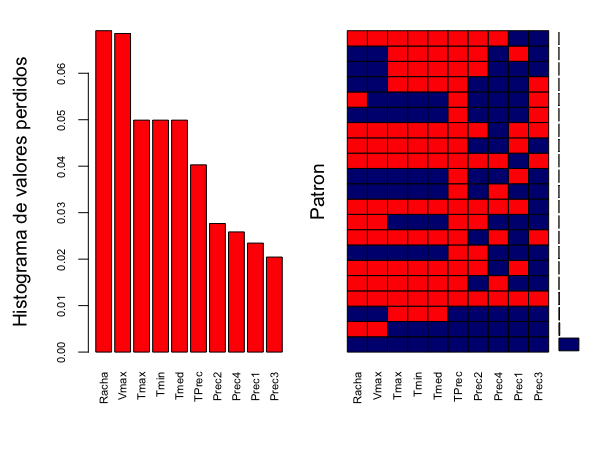
\includegraphics[scale=0.6]{./Capitulo2/imagenes/perdidos.png}
		\caption{Patr�n e histograma de valores perdidos.}
	\label{perdidos}
\end{figure}

Acorde a los resultados de la figura anterior, no podemos concluir que haya un patr�n claro pero si podemos asegurar que cuando Tmax tiene un valor perdido las dem�s tambi�n lo tendr�n con probabilidad por lo que utilizar regresiones ser� quiz� mala soluci�n, por ello nos decantaremos por el m�todo \textbf{pmm} del paquete MICE. Tras lo cual, tendremos el dataset con una cantidad 0 de valores perdidos en Tmax. 

\section{Agregaci�n}

Este paso del preprocesado es solo necesario para la soluci�n del problema mensual. Para ello, usaremos el comando aggregate y la funci�n max para agregar para cada mes de cada a�o la mayor temperatura registrada de manera que podamos realizar predicciones y modelado de serie a nivel mensual. Para poder realizar esto, previamente hemos pasado la fecha de tipo string a tipo date y tras ello, hemos eliminado el d�a de la fecha de manera que podemos agregar por las parejas iguales de mes y a�o. 
\pagebreak
\clearpage
%---------------------------------------------------